Liang et al. \cite{liangLearningNonLocalSpatialAngular2023a} propose the Epipolar Transformer model (EPIT),
for the task of light field super resolution.
The authors aim to improve the exploitation of spatial-angular correlation.
To this end a $4$d light field $X \in \mathbb R^{U \times V \times W \times H \times C}$ 
is mapped onto multiple $2$d epipolar plane images $E^{(b)} \in \mathbb R^{V \times W \times C}$, for $b = 1, ..., HW$.
The EPI is flattened along the first and second dimension and treated as a sequence $(x_k^{(b)})_{k=1}^{VW} \in \mathcal S (\mathbb R^C)$.
Then the self-attention mechanism is employed, 
in order to learn the long range spatial-angular correlation along the epipolar line.
The overall architecture is depicted in figure \ref{fig:epit}.

\begin{figure}[h!]
    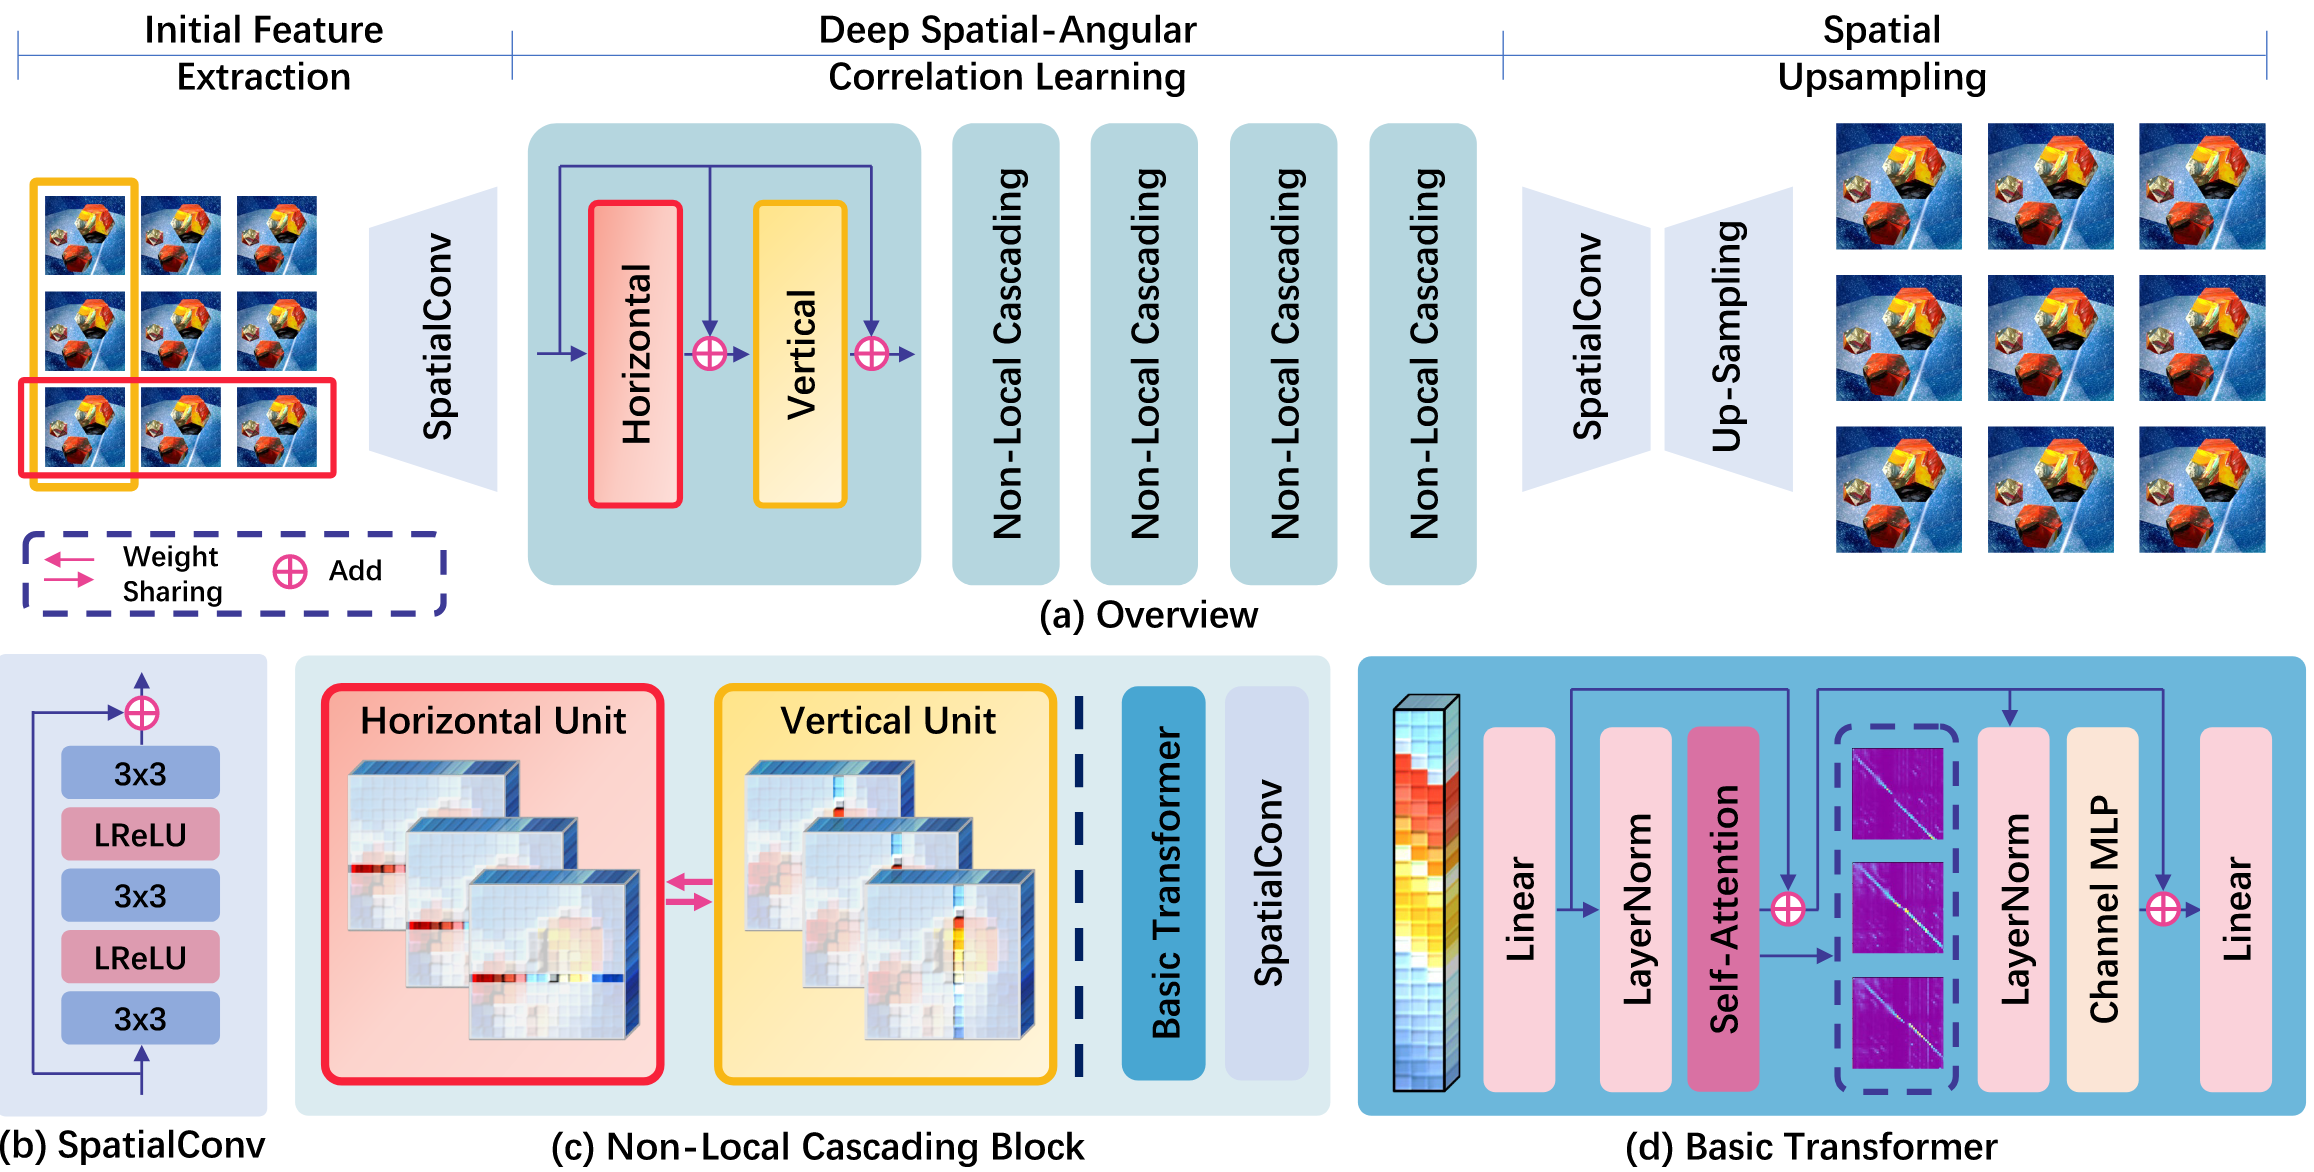
\includegraphics[width=0.9\textwidth]{models/lfsr/imgs/epit.png}
    \caption{Image taken from \cite{caiMSTMultistageSpectralwise2022a}, architecture of EPIT model.}
    \label{fig:epit}
\end{figure}

The deep feature extraction model $H_d$ proposed by Liang et al. \cite{liangLearningNonLocalSpatialAngular2023a}, consists of $5$ Non-Local Cascading Blocks (NLCBs)

    $$ H_d = H_{NLCB} \circ ... \circ H_{NLCB} ~.$$

The NLCB is composed of a horizontal and a vertical unit,
to extract features along the horizontal epipolar line, 
and the vertical epipolar line respectively. 
Additionally, each unit is followed by a shallow convolutional network, 
both encapsuled inside of a residual connection, that is

    $$H_{NCLB} = R(C_{SpaConv} \circ H_v) \circ R(C_{SpaConv} \circ H_h) ~.$$

The spatial convolution is made up of three cascaded convolutions, 
interspersed by leaky ReLU activation functions with a negative slope of $0.2$

    $$ C_{SpaConv} = C \circ \text{LReLU}(0.2) \circ C \circ \text{LReLU}(0.2) \circ C ~,$$

where $C = C(64, 64)$.
We explain the construction of the horizontal unit $H_h$ in greater detail,
that of $H_v$ is analog to it.
Given an input $X \in \mathbb R^{U \times V \times H \times W \times C}$,
the second and third dimension are transposed, 
and it is reshaped to $UH \times VW \times C$,
capturing this in form of an operation gives us

    $$\pi_h = \Pi_{U \times H \times V \times W \times C}^{UH \times VW \times C} \circ P_{\sigma_{SAI \to EPIH}} ~.$$

The first dimension is treated as the batch dimension, 
while the second as the sequence length.
The sequences are then processed by a transformer block with $8$ heads and a dimension of $128$,
formally that is

    $$ H_{h} =  \pi_h^{-1} \circ T(128, 8, \Phi) \circ \pi_h ~.$$

For the mapping $\Phi$ a two layer neural network is employed

    $$ \Phi = F(128, 64) \circ \text{ReLU} \circ F(64, 128) ~.$$

The vertical unit is constructed analogously

    $$ H_v = \pi_v^{-1} \circ T(128, 8, \Phi) \circ \pi_v ~, $$

where $\pi_v = \Pi_{V \times W \times U \times H \times C}^{VW \times UH \times C} \circ P_{\sigma_{SAI \to EPIV}}$.
The weights of the transformer block $T$ of the horizontal and the vertical unit of each NLCB are shared.
